%%%%%%%%%%%%%%%%%%%%%%%%%%%%%%%%%%%%%%%%%%%%%%%%
%% Intro to LaTeX and Template for Homework Assignments
%% Quantitative Methods in Political Science
%% University of Mannheim
%% Fall 2018
%%%%%%%%%%%%%%%%%%%%%%%%%%%%%%%%%%%%%%%%%%%%%%%%

% created by Marcel Neunhoeffer & Sebastian Sternberg

% COMMANDS: 
	% To do anything in LaTeX, you must use commands
	% Commands tell LaTeX when to start your document, how you want your document to look, and how to format your document
	% Commands ALWAYS begin with a backslash \

% Everything following the % sign is a comment and will not be used by Latex to compile your document.
% This is very similar to # comments in R.

% Every .tex file usually consists of four parts.
% 1. Document Class
% 2. Packages
% 3. Header
% 4. Your Document
 
\documentclass[a4paper,12pt]{article} % This defines the style of your paper

%%%%%%%%%%%%%%%%%%%%%%%%%%%%%%%%%%%%%%%%%%%%%%%%
% 2. Packages
%%%%%%%%%%%%%%%%%%%%%%%%%%%%%%%%%%%%%%%%%%%%%%%%

% Packages are libraries of commands that LaTeX can call when compiling the document. With the specialized commands you can customize the formatting of your document.
% If the packages we call are not installed yet, TeXworks will ask you to install the necessary packages while compiling.

% First, we usually want to set the margins of our document. For this we use the package geometry. We call the package with the \usepackage command. The package goes in the {}, the parameters again go into the [].
\usepackage[top = 2.5cm, bottom = 2.5cm, left = 2.5cm, right = 2.5cm]{geometry} 
\usepackage[T1]{fontenc}
\usepackage[utf8]{inputenc}
\usepackage{hyperref}
\usepackage{tikz} %for the flow chart
\usetikzlibrary{shapes,arrows}
\usepackage{amsmath} %math package
\usepackage{amsmath, nccmath} %multiple fractions
\usepackage{pgfplots} %plots
\usepackage{pgfplotstable} %to plot from imported text files
\pgfplotsset{compat = newest}
\usepackage{subcaption} %figures with multiple captions
\usepackage{multirow} % Multirow is for tables with multiple rows within one cell.
\usepackage{booktabs} % For even nicer tables.
\usepackage{graphicx} %to include some plots (.pdf files) we need a package for that.
\usepackage[justification=centering]{caption} %Centering captions under the figures
\usepackage{setspace}
\setlength{\parindent}{0in} %The following command sets the indent to 0.
\usepackage{float} % Package to place figures where you want them.
\usepackage{fancyhdr} % to create nice headers.
\usepackage[numbered, framed]{mcode} %Package for Matlab code listings:
\lstset{stepnumber  = 5, % Line numbers go in steps of 4
	breaklines  = true,
	breakautoindent=true, 
	breakindent=10pt,
	breakatwhitespace   = false,
	prebreak= \space,
	postbreak   = \space}


%%%%%%%%%%%%%%%%%%%%%%%%%%%%%%%%%%%%%%%%%%%%%%%%
% 3. Header (and Footer)
%%%%%%%%%%%%%%%%%%%%%%%%%%%%%%%%%%%%%%%%%%%%%%%%
\pagestyle{fancy} % % To make our document nice we want a header and number the pages in the footer. With this command we can customize the header style.
\fancyhf{} % This makes sure we do not have other information in our header or footer.
\lhead{\footnotesize Agent-based Modelling}% \lhead puts text in the top left corner. \footnotesize sets our font to a smaller size. \rhead works just like \lhead (you can also use \chead)
\rhead{\footnotesize Christopher Golling, Gael Mourouga, Author 3, Author 4, Author 5} %<---- Fill in your lastnames.
\cfoot{\footnotesize \thepage} % We want to put our page number in the center.

%%%%%%%%%%%%%%%%%%%%%%%%%%%%%%%%%%%%%%%%%%%%%%%%
% 4. document
%%%%%%%%%%%%%%%%%%%%%%%%%%%%%%%%%%%%%%%%%%%%%%%%

\begin{document}

\thispagestyle{empty} % This command disables the header on the first page. 
\begin{tabular}{p{15.5cm}} % This is a simple tabular environment to align your text nicely 
%---------
{\large \bf Agent-based Modelling} \\
Fall 2021  \\
\hline % \hline produces horizontal lines.
\\
\end{tabular} % Our tabular environment ends here.
%--------------
\vspace*{0.3cm} % some vertical space in between the line and our title.

%----------------------------Title
\begin{center} % Everything within the center environment is centered.
	{\Large \bf Coding Project: Crop Wars}
	\vspace{2mm}
	
        % YOUR NAMES GO HERE
	{\bf Christopher Golling, Gael Mourouga, Aaron Moser, Author 4, Author 5 } % <---- Fill in your names here!
		
\end{center}  
%-----------------------------
%%%%%%%%%%%%%%%%%%%%%%%%%%%%%%%%%%%%%%%%%%%%%%%%
%%%%%%%%%%%%%%%%%%%%%%%%%%%%%%%%%%%%%%%%%%%%%%%%

\vspace{0.4cm}

%----------------First section
\section{Introduction}

Agricultural structures are shaped by a variety of factors, including economic, environmental, cultural, technological and geographical conditions \cite{happeAgriculturalPoliciesFarm2004}. \\
Consequently, both farmers and policymakers can benefit from farm-level models which optimise water usage and crop nature, based on a set of different externalities including water ressources availability and market dynamics.\\
The model featured in this coding project aims to illustrate the process behind the development of agent-based farm-level models, by starting with a simple, deterministic model that is progressively complexified with elements from physics-based models and game theory.


\section{State-of-the-Art}

To guide the development of our illustrative model, a literature review was conducted to assess the state-of-the-art on agent-based modelling for water ressources allocation and farming simulations. \\
Our starting point was the thesis \textit{"Agricultural policies and farm structures: Agent-based modelling and application to EU-policy reform"} by Happe (2004) \cite{happeAgriculturalPoliciesFarm2004}, which outlines in details the development of an agent-based model (AgriPoliS) to assess the influence of agricultural policies at the farm level, which is applied to a case study in the region of Holenhole in Germany.\\
To have an overview of more recent approaches. a seed review paper was selected, \textit{"A review of Agent Based Modeling for agricultural policy evaluation"} by Kremmydas et al.(2018) \cite{kremmydasReviewAgentBased2018} from which a literature graph was generated using the online tools \href{https://www.connectedpapers.com/main/35fac7b643317e5f48f5280fadec94051bf2401f/A-review-of-Agent-Based-Modeling-for-agricultural-policy-evaluation/graph}{Connected Papers}, and is analysed on figure \ref{fig:State_of_the_art}.\\
For completeness, the graphs generated through other seed papers were also analysed, including an older paper applying game theory to decision making in farmer cooperatives by Staatz (1983) \cite{staatzGametheoreticAnalysisDecision1983} and a case application of agent-based models to water allocation on the transboundary Nile river by Ding (2016) \cite{dingAgentBasedModelling2016}.


\begin{figure}[H]
	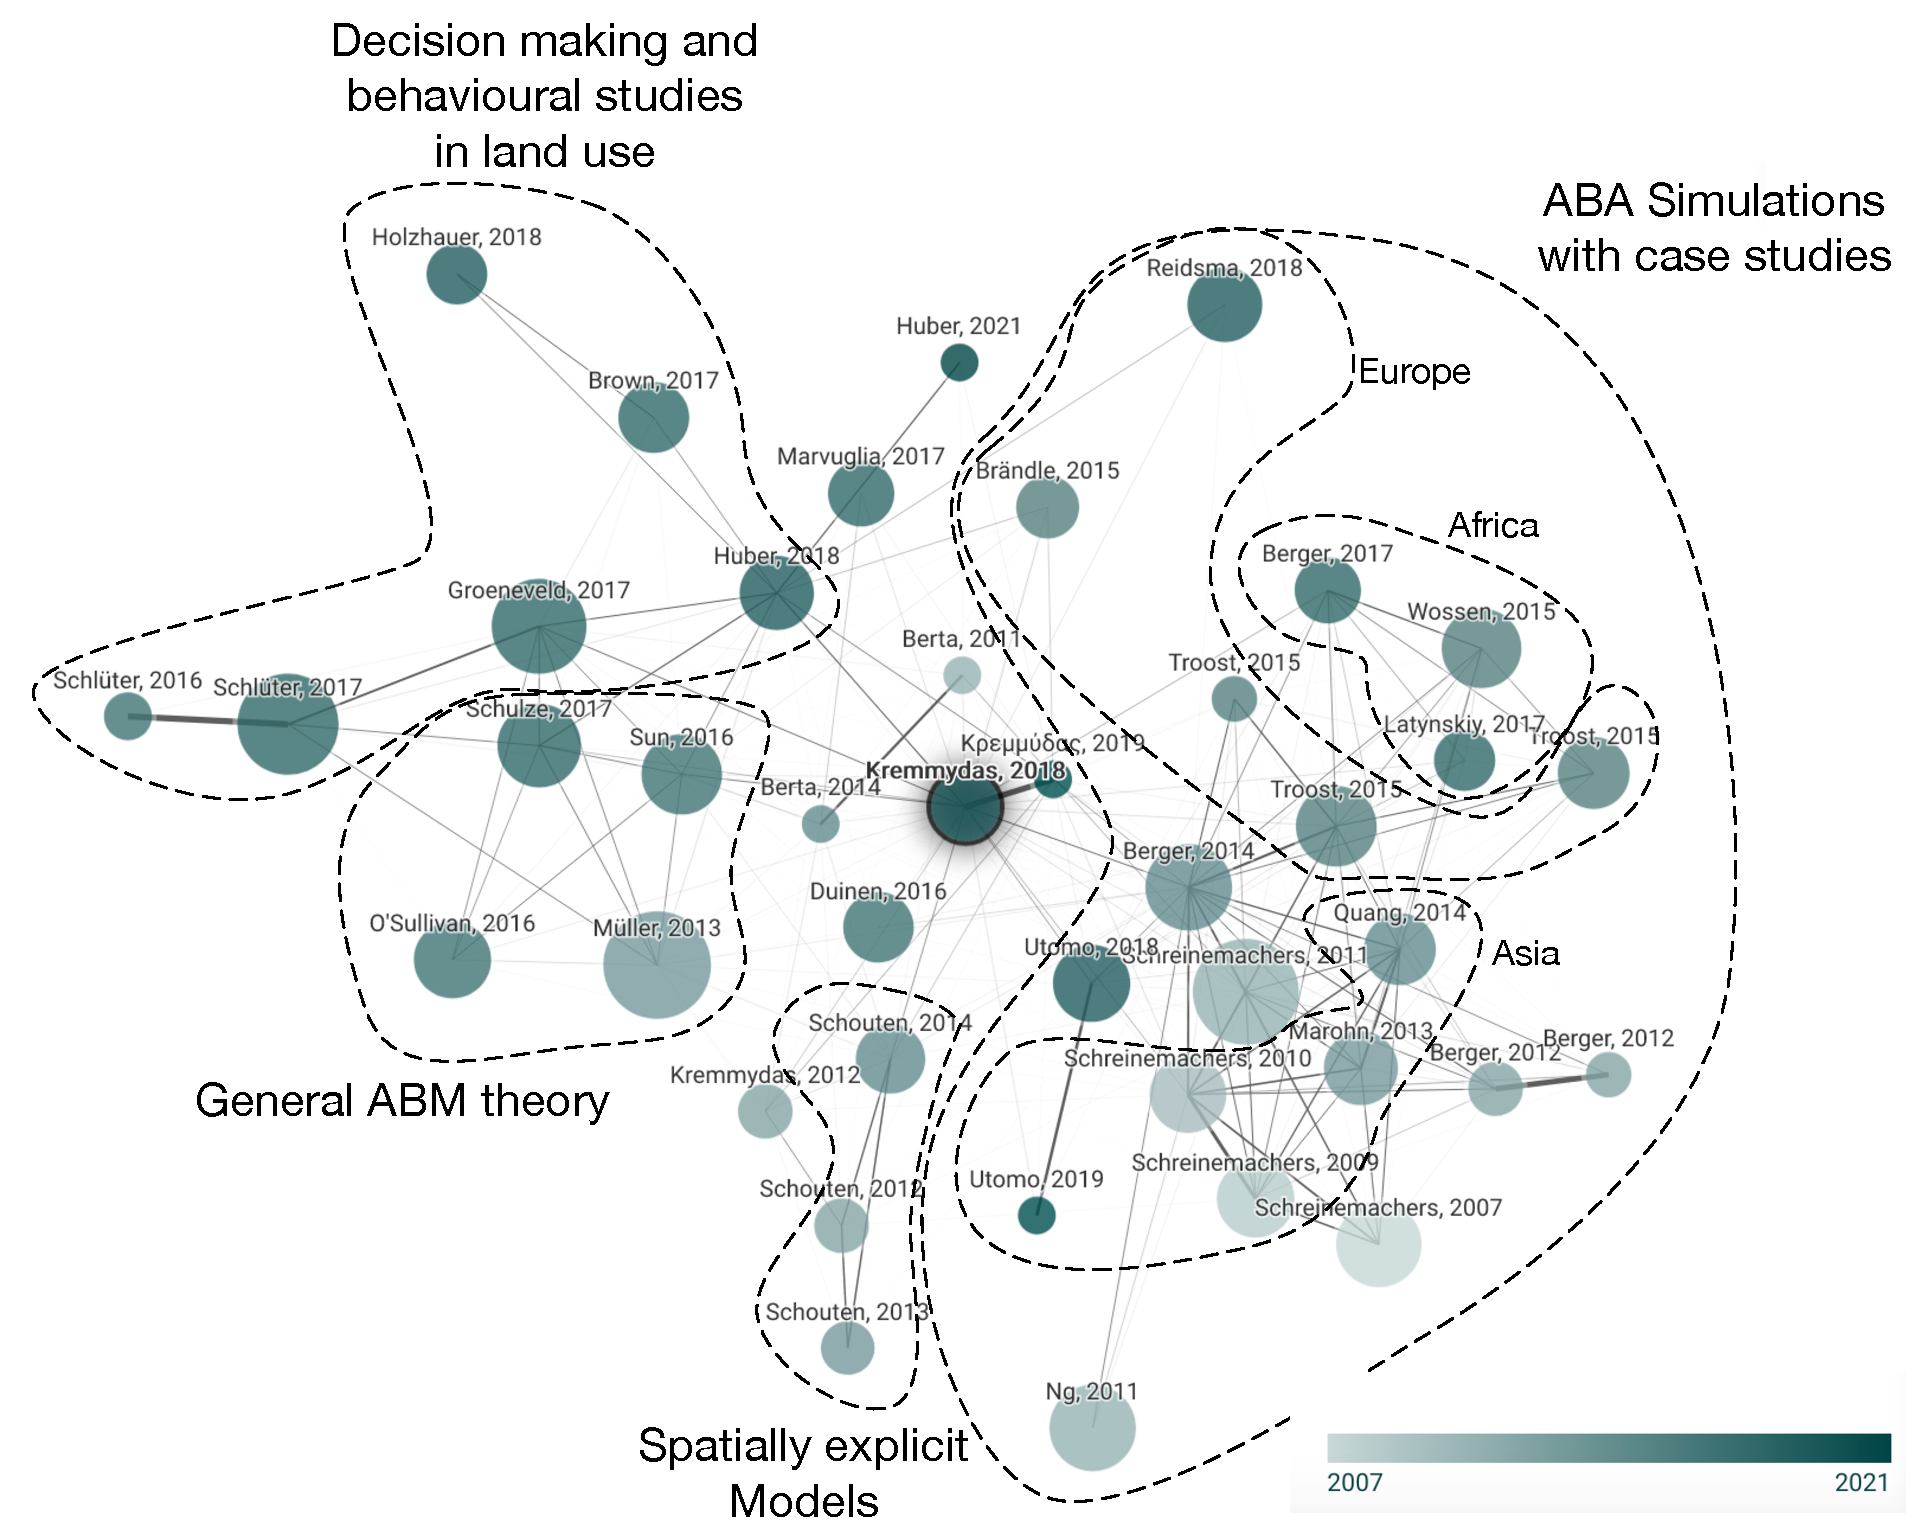
\includegraphics[width=\textwidth]{Figures/StateOfTheArt2.pdf}
	\centering
	\caption{Graph showing papers related to ref.X generated on ConnectedPapers.com. Circle radius is proportionnal to number of citation, color to publication date, dashed line refers to paper categories.}
	\label{fig:State_of_the_art}
\end{figure}

\newpage
\bibliographystyle{ieeetr} 
\bibliography{AgentBasedModelling.bib}

\end{document}
